\documentclass{beamer}
\usetheme{Madrid}
\useinnertheme{rounded}
\usecolortheme{whale}

\title{Next Reaction Method}
\subtitle{Efficient Stochastic Simulation of Chemical Systems}
\author{Lorenzo Beretta}
\date{29th July 2019}

%pacchetti scrittura
\usepackage{dsfont}
\usepackage{amsthm}
\usepackage{amsmath}
\usepackage{amssymb}
\usepackage{mathrsfs}
\usepackage{mathtools}
\usepackage{enumitem}
\usepackage{hyperref}
\usepackage{marginnote}
\usepackage{scalerel}
\usepackage{comment}
\usepackage[utf8]{inputenc}

%% miei %%
\usepackage{tkz-graph}
\usepackage{algorithm,algorithmic}
\usepackage{tikz}
\usepackage{color}
\usepackage{centernot}
\usepackage{esvect}
\newcommand{\labelenumi}{\arabic{enumi}.} 
\newcommand{\labelenumii}{\roman{enumii}.}
\DeclareMathOperator{\Exp}{\text{Exp}}
\DeclareMathOperator*{\argmin}{arg\,min}
\setbeamertemplate{items}[square]
\usetikzlibrary{matrix}

% tikz
\usetikzlibrary{positioning,chains,fit,shapes,calc}
\definecolor{myblue}{RGB}{80,80,160}
\definecolor{mygreen}{RGB}{80,160,80}

\usetikzlibrary{shapes.misc}
\usetikzlibrary{shapes.symbols}
%\usetikzlibrary{snakes}
\usetikzlibrary{decorations}
\usetikzlibrary{decorations.markings}

%%%%%%%%%%%%%%%%%%%%%%%%%%%%%%%%%%%%%%%%%%%%%%%%%%%%%%%%%%%%%%%%%%%%%%%%%%%%%%%%%%%%%%%%%%%%%%%%%%%%%%%%
\usepackage{marginnote}
\usepackage{scalerel} % to rescale the paraproduct symbols
%%%
%% copied from here
\usepackage{tikz}



\colorlet{symbols}{black}
\colorlet{testcolor}{green!60!black}


\def\symbol#1{\textcolor{symbols}{#1}}
\def\1{\mathbf{{1}}}
\def\X{\symbol{X}}
\def\Wick#1{\,\colon\!\! \phantom{1} #1 \phantom{1} \!\colon}

\def\drawx{\draw[-,solid] (-3pt,-3pt) -- (3pt,3pt);\draw[-,solid] (-3pt,3pt) -- (3pt,-3pt);}
\tikzset{
	root/.style={circle,fill=gray,inner sep=0pt, minimum size=2mm},
	dot/.style={circle,fill=black,inner sep=0pt, minimum size=1mm},
	var/.style={circle,fill=black!10,draw=black,inner sep=0pt, minimum size=2mm},
	circ/.style={circle,fill=white,draw=black,inner sep=0pt, minimum size=1.2mm},
	dotred/.style={circle,fill=black!50,inner sep=0pt, minimum size=2mm},
	generic/.style={semithick,shorten >=1pt,shorten <=1pt},
	gepsilon/.style={semithick,shorten >=1pt,shorten <=1pt,densely dashed},
	dist/.style={ultra thick,draw=testcolor,shorten >=1pt,shorten <=1pt},
	testfcn/.style={ultra thick,testcolor,shorten >=1pt,shorten <=1pt,<-},
	testfcnx/.style={ultra thick,testcolor,shorten >=1pt,shorten <=1pt,<-,
		postaction={decorate,decoration={markings,mark=at position 0.6 with {\drawx}}}},
	kprime/.style={semithick,shorten >=1pt,shorten <=1pt,dotted,->},
	kprimex/.style={semithick,shorten >=1pt,shorten <=1pt,densely dashed,->,
		postaction={decorate,decoration={markings,mark=at position 0.4 with {\drawx}}}},
	kernel/.style={semithick,shorten >=1pt,shorten <=1pt,->},
	multx/.style={shorten >=1pt,shorten <=1pt,
		postaction={decorate,decoration={markings,mark=at position 0.5 with {\drawx}}}},
	kernelx/.style={semithick,shorten >=1pt,shorten <=1pt,->,
		postaction={decorate,decoration={markings,mark=at position 0.4 with {\drawx}}}},
	kepsilon/.style={semithick,shorten >=1pt,shorten <=1pt,densely dashed,->},
	kernel1/.style={->,semithick,shorten >=1pt,shorten <=1pt,postaction={decorate,decoration={markings,mark=at position 0.45 with {\draw[-] (0,-0.1) -- (0,0.1);}}}},
	kernel2/.style={->,semithick,shorten >=1pt,shorten <=1pt,postaction={decorate,decoration={markings,mark=at position 0.45 with {\draw[-] (0.05,-0.1) -- (0.05,0.1);\draw[-] (-0.05,-0.1) -- (-0.05,0.1);}}}},
	kernelBig/.style={semithick,shorten >=1pt,shorten <=1pt,decorate, decoration={zigzag,amplitude=1.5pt,segment length = 3pt,pre length=2pt,post length=2pt}},
	rho/.style={dotted,semithick,shorten >=1pt,shorten <=1pt},
	renorm/.style={shape=circle,fill=white,inner sep=1pt},
	labl/.style={shape=rectangle,fill=white,inner sep=1pt},
	xi/.style={circle,fill=symbols!10,draw=symbols,inner sep=0pt,minimum size=1.2mm},
	xix/.style={crosscircle,fill=symbols!10,draw=symbols,inner sep=0pt,minimum size=1.2mm},
	xib/.style={circle,fill=symbols!10,draw=symbols,inner sep=0pt,minimum size=1.6mm},
	xibx/.style={crosscircle,fill=symbols!10,draw=symbols,inner sep=0pt,minimum size=1.6mm},
	not/.style={circle,fill=symbols,draw=symbols,inner sep=0pt,minimum size=0.5mm},
	>=stealth,
	}

\makeatletter
\def\DeclareSymbol#1#2#3{\expandafter\gdef\csname MH@symb@#1\endcsname{\tikz[baseline=#2,scale=0.15,draw=symbols]{#3}}\expandafter\gdef\csname MH@symb@#1s\endcsname{\scalebox{0.7}{\tikz[baseline=#2,scale=0.15,draw=symbols]{#3}}}}
\def\<#1>{\csname MH@symb@#1\endcsname}
\makeatother

\DeclareSymbol{1}{0}{\draw[white] (-.4,0) -- (.4,0); \draw (0,0)  -- (0,1.2) node[dot] {};}
\DeclareSymbol{2}{0}{\draw (-0.5,1.2) node[dot] {} -- (0,0) -- (0.5,1.2) node[dot] {};}
\DeclareSymbol{3}{0}{\draw (0,0) -- (0,1.2) node[dot] {}; \draw (-.7,1) node[dot] {} -- (0,0) -- (.7,1) node[dot] {};}
\DeclareSymbol{30}{-3}{\draw (0,0) -- (0,-1); \draw (0,0) -- (0,1.2) node[dot] {}; \draw (-.7,1) node[dot] {} -- (0,0) -- (.7,1) node[dot] {};}
\DeclareSymbol{31}{-3}{\draw (0,0) -- (0,-1) -- (1,0) node[dot] {}; \draw (0,0) -- (0,1.2) node[dot] {}; \draw (-.7,1) node[dot] {} -- (0,0) -- (.7,1) node[dot] {};}
\DeclareSymbol{32}{-3}{\draw (0,0) -- (0,-1) -- (1,0) node[dot] {}; \draw (0,0) -- (0,-1) -- (-1,0) node[dot] {}; \draw (0,0) -- (0,1.2) node[dot] {}; \draw (-.7,1) node[dot] {} -- (0,0) -- (.7,1) node[dot] {};}
\DeclareSymbol{20}{-3}{\draw (0,0) -- (0,-1);\draw (-.7,1) node[dot] {} -- (0,0) -- (.7,1) node[dot] {};}
\DeclareSymbol{22}{-3}{\draw (0,0.3) -- (0,-1) -- (1,0) node[dot] {}; \draw (0,0.3) -- (0,-1) -- (-1,0) node[dot] {};\draw (-.7,1) node[dot] {} -- (0,0.3) -- (.7,1) node[dot] {};}
\DeclareSymbol{31p}{-3}{\draw (0,0) -- (0,-1) -- (1,0) node[dot] {}; \draw (0,0) -- (0,1.2) node[dot] {}; \draw (-.7,1) node[dot] {} -- (0,0) -- (.7,1) node[dot] {}; \draw (0,-1) node{\scaleobj{0.5}{\pe}}; }
\DeclareSymbol{32p}{-3}{\draw (0,0) -- (0,-1) -- (1,0) node[dot] {}; \draw (0,0) -- (0,-1) -- (-1,0) node[dot] {}; \draw (0,0) -- (0,1.2) node[dot] {}; \draw (-.7,1) node[dot] {} -- (0,0) -- (.7,1) node[dot] {}; \draw (0,-1) node{\scaleobj{0.5}{\pe}};}
\DeclareSymbol{22p}{-3}{\draw (0,0.3) -- (0,-1) -- (1,0) node[dot] {}; \draw (0,0.3) -- (0,-1) -- (-1,0) node[dot] {};\draw (-.7,1) node[dot] {} -- (0,0.3) -- (.7,1) node[dot] {}; \draw (0,-1) node{\scaleobj{0.5}{\pe}};}

\usepackage{forest}
\usepackage{comment}
\usetikzlibrary{decorations.pathreplacing}


%%%%%%%%%%%%%%%%%%%%%%%%%%%%%%%%%%%%%%%%%%%%%%%%%%%%%%%%%%%%%%%%%%%%%%%%%%%%%%%%%%%%%%%%%%%%%%%%

\begin{document}

\begin{frame}
  \maketitle
\end{frame}

\begin{frame}{Predictive Model Definition}
  To define a predictive model we need two steps:
  \begin{itemize}
  \item $\bullet$ Define a descriptive model of the phenomenon
    \begin{block}{Descriptive Model: Differential Equation}
      The Newton's law of motion:
      $$ \vv{F} = m \, \frac{\partial^2 \vv{x}}{\partial t^2} $$
    \end{block}    
  \item $\bullet$ Define a computational model to make predictions
    \begin{block}{Computational Model: Numerical Integration}
      \begin{figure}[h]
        \centering
        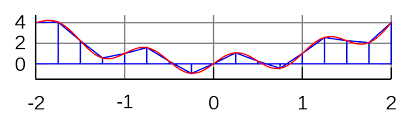
\includegraphics[scale=0.6]{num_int}
      \end{figure}
    \end{block}
  \end{itemize}
\end{frame}

\begin{frame}{Coupled Chemical System: Mathematical Description}
  \begin{columns}
    \begin{column}{.45 \textwidth}
      \begin{block}{Set of Elementary Reactions}
        \begin{equation*}
          \begin{gathered}
            A + B \rightarrow C \\
            B + C \rightarrow D \\
            D + E \rightarrow E + F \\
            F \rightarrow D + G \\
            E + G \rightarrow A   
          \end{gathered}
        \end{equation*}
      \end{block}
    \end{column}
    \begin{column}{.45 \textwidth}
      \begin{block}{Model Assumptions}
        \begin{itemize}
        \item $\bullet$ Many molecules: continuous and deterministic
        \item $\bullet$ Few molecules:\\ discrete and stochastic
        \end{itemize}
      \end{block}
    \end{column}
  \end{columns}
\end{frame}


\begin{frame}{Deterministic Framework}
  \begin{columns}
    \begin{column}{.45 \textwidth}
      \begin{block}{Set of Elementary Reactions}
        \begin{equation*}
          \begin{gathered}
            A + B \rightarrow C \\
            B + C \rightarrow D \\
            D + E \rightarrow E + F \\
            F \rightarrow D + G \\
            E + G \rightarrow A   
          \end{gathered}
        \end{equation*}
      \end{block}
    \end{column}
    \begin{column}{.45 \textwidth}
      \begin{block}{Computation}
        \begin{equation*}
          \begin{gathered}
            \frac{\partial [A]}{\partial t} = f_A\left([A], \dots [G]\right) \\
            \frac{\partial [B]}{\partial t} = f_B\left([A], \dots [G]\right) 
            \vdots\\
            \frac{\partial [G]}{\partial t} = f_G\left([A], \dots [G]\right)
          \end{gathered}
        \end{equation*}
      \end{block}
    \end{column}
  \end{columns}
\end{frame}

\begin{frame}{Stochastic Framework}
  \begin{columns}
    \begin{column}{.45 \textwidth}
      \begin{block}{Set of Elementary Reactions}
        \begin{equation*}
          \begin{gathered}
            R_1 + R^\prime_2 \xrightarrow{k_1} P_1 \\
            R_2 + R^\prime_2 \xrightarrow{k_2} P_2 \\
            R_3 + R_3^\prime \xrightarrow{k_3} P_3 + P_3^\prime 
          \end{gathered}
        \end{equation*}
      \end{block}
    \end{column} 
    \begin{column}{.45 \textwidth}
      \begin{block}{Propensity $k_i$}
        The probability that $i$-th reaction occurs
        in  $[0, dt]$ is
        $$k_i dt + o(dt)$$
        fixing molecules IDs a priori.
      \end{block}
    \end{column}
  \end{columns}
  \begin{block}{Reaction Rate $a_i$}
    The probability that $i$-th reaction occurs
    in  $[0, dt]$ is
    $$a_i dt + o(dt)$$
    with
    $$ a_i = k_i \cdot \# R_1 \dots \#R_n$$
  \end{block}
\end{frame}

\begin{frame}{Stochastic Framework}
  \begin{block}{Model Assumptions}
    \begin{itemize}
    \item $\bullet$ Molecules in solution $\implies$ No position $\implies$ States are multisets
      \begin{center}
        \begin{minipage}{.7 \textwidth}
          \begin{block}{State}
            $$ S = \left\{ \#M_1, \, \dots \#M_m \right\} $$
          \end{block}
        \end{minipage}
      \end{center}
      \vspace{1.pt}
    \item $\bullet$ Propensities are constant 
      \begin{center} 
       \begin{minipage}{.7 \textwidth}
          \begin{block}{Transition Probability}
            If $a_1$ reaction turns $S$ into $S^\prime$, then for each $t > 0$
            $$ \mathbb{P}\left(S^\prime, t + dt \,  \middle| \, S, t \right) = a_1dt + o(dt) $$
          \end{block}
        \end{minipage}
      \end{center}   
    \end{itemize}
  \end{block}
\end{frame}

\begin{frame}{How to Compute the Solution?}
  The model is finite state CTMC , solved exactly by
  \begin{block}{Master Equation}
    \begin{itemize}
    \item $\bullet$ One variable $p_S$ per state $S$
    \item $\bullet$ transition probabilities $\longrightarrow$ differential equations 
    \item $\bullet$ Exponential number of states $\implies$ intractable problem
    \end{itemize}
  \end{block}
  
  \begin{block}{Monte Carlo simulation}
    \begin{itemize}
    \item $\bullet$ Sample unbiased trajectories
    \item $\bullet$ Markov property simplifies computation
    \item $\bullet$ Gillespie's \textbf{Direct Method} and \textbf{First Reaction Method} 
    \end{itemize}
  \end{block}
\end{frame}

\begin{frame}{Reaction Times Distribution}
  Let $f:\left[0, +\infty\right) \longrightarrow \mathbb{R}^+$ density of $i$-th reaction's time 
  \begin{equation*}
    \left\{
    \begin{aligned}
      &f(0) = \frac{d}{dt} \mathbb{P}_i \left(dt \, \middle| \, S, 0 \right)= a_i\\
      &f(t + t_0) = \frac{f(t)}{1 - \int_0^{t_0} f(s)\, ds}         
    \end{aligned}\right.
    \implies f(t) =  a_i e^{-a_i t}
  \end{equation*}
  \begin{block}{Exponential Distribution}
    \begin{itemize}
    \item $\bullet$ The $i$-th reaction time is distributed as $\Exp(a_i)$
    \item $\bullet$ $\Exp(a_1) \land \dots \land \Exp(a_n)$ is distributed as
      $\Exp\left(\sum_{i\leq n} a_i\right)$ 
    \item $\bullet$ Reactions happen as hitting times of an homogeneous 
      $$\text{\textbf{Poisson Process} of rate } \lambda =  \sum_{i\leq n} a_i$$ 
    \end{itemize}
  \end{block}
\end{frame}

\begin{frame}{Gillespie's Direct Method}
  \begin{block}{Lemma}
    Given $\left\{\Exp(a_j)\right\}_{j\leq n}$ independent 
    \begin{equation*}
      \mathbb{P}\left[Exp(a_i) \leq \Exp(a_j) \; \forall j \leq n \right] = \frac{a_i}{\sum_ja_j}
    \end{equation*}
  \end{block}
  \begin{block}{Direct Method}
    \begin{enumerate}
    \item Initialize $S$ and $t\leftarrow 0$ 
    \item Calculate $a_i$ for each reaction $i$
    \item Sample reaction $\mu$ with probability $a_\mu \big/ \sum_j a_j$
    \item Sample $\tau$ from distribution $\Exp\left(\sum_j a_j\right)$
    \item Update $S$ and $t \leftarrow t + \tau$
    \item Go to step 2.
    \end{enumerate}
  \end{block}
\end{frame}

\begin{frame}{Gillespie's First Reaction Method}
  \begin{block}{First Reaction Method}
    \begin{enumerate}
    \item Initialize $S$ and $t\leftarrow 0$ 
    \item Calculate $a_i$ for each reaction $i$
    \item For each reaction $i$: \\
      $\quad$ Sample a \textbf{tentative time} $\tau_i$ from $\Exp\left(a_i\right)$  
    \item Define $\mu = \argmin\limits_i\left\{\tau_i\right\}$ and $\tau = \tau_\mu$
    \item Update $S$ and $t \leftarrow t + \tau$
    \item Go to step 2.
    \end{enumerate}
  \end{block}
  \begin{block}{Method Equivalence}
    \begin{itemize}
    \item $\bullet$ $\Exp(a_1) \land \dots \land \Exp(a_n) \sim
      \Exp\left(\sum_{i\leq n} a_i\right) \implies \tau_{DM}  \sim \tau_{FRM}$
    \item $\bullet$ $\mathbb{P}\left[Exp(a_i) \leq \Exp(a_j) \;
        \forall j \leq n \right] = a_i \big/\sum_ja_j \implies \mu_{DM} \sim \mu_{FRM}$
    \end{itemize}
  \end{block}
\end{frame}

\begin{frame}{Gillespie's Methods}
  \begin{block}{Unbiased Estimators}
    DM and FRM are unbiased estimators of
    master equation solution

  \end{block}
  \begin{block}{Naive Implementations Comparison}
    \begin{itemize} 
    \item $\bullet$ Direct Method samples 2 random numbers
    \item $\bullet$ The First Reaction Method samples one per reaction 
    \item $\bullet$ RNG takes up to 10x FLOP
    \end{itemize}
  \end{block}
\center \Huge{SLIDE DA CAMBIARE}
\end{frame}

\begin{frame}{Next Reaction Method}
  \begin{block}{Optimize First Reaction Method}
    \begin{itemize}
    \item $\bullet$ Store and reuse Random Generated Numbers
    \item $\bullet$ Minimize $a_i$ and $\tau_i$ recalculations
    \item $\bullet$ Appropriate data structure to store $\bigl\{\tau_i\bigr\}_i$
    \end{itemize}
  \end{block}
  \begin{block}{Dependency Graph}
    $G=\left(V,\, E\right)$ where $V$ are reactions \\
    \vspace{2pt}
    For each reaction $u,\, v \in V$:
    \begin{itemize}
    \item $\bullet$ \textsc{Affects}$(u) \simeq $ \textsc{Reactants}$(u)$ $\cup$ \textsc{Products}$(u)$
    \item $\bullet$ \textsc{DependsOn}$(v) \simeq $ \textsc{Reactants}$(v)$
    \item $\bullet$ \textsc{Affects}$(u)$ $\cap$
      \textsc{Reactants}$(v) \neq \emptyset$ $\iff \bigl(u, v \bigr) \in E$   
    \end{itemize}    
  \end{block}
\end{frame}

\begin{frame}{Indexed Priority Queue}
  \begin{block}{Data Structure}
    We need to store key-value pairs $\left(\tau_i,\, i\right)$ supporting:
    \begin{itemize}
    \item $\bullet$ \textsc{PopMin}
    \item $\bullet$ \textsc{UpdateKey}
    \end{itemize}
  \end{block}
  \vspace{5pt}
  Dependency Graph sparse $\implies$ few calls to \textsc{UpdateKey}
  \begin{center}
    \textbf{Priority Queue $\pmb{\gg}$ Array}
  \end{center}
  Naive PQ: \textsc{UpdateKey} = \textsc{DeleteKey} + \textsc{InsertKey}
\end{frame}

\begin{frame}{Indexed Priority Queue: \textsc{Updatekey}}
  \begin{columns}
    \begin{column}{0.7 \textwidth}
      
        \begin{forest}
          for tree={rectangle,draw, align=center, l sep=20pt, minimum size=3.2em}
          [{A \\ $\left[\tau_4, 4\right]$}, 
          [{B \\ $\left[\tau_1, 1\right]$}
          [{D \\ $\left[\tau_6, 6\right]$}
          [{H \\ $\left[\tau_7, 7\right]$}]
          [{I \\ $\left[\tau_5, 5\right]$}]
          ] 
          [{E \\ $\left[\tau_0, 0\right]$}]
          ]
          [{C \\ $\left[\tau_2, 2\right]$}, fill=green
          [{F \\ $\left[\tau_3, 3\right]$}
          [{L \\ $\left[\tau_8, 8\right]$}]
          ]  
          [{G \\ $\left[\tau_{9}, 9\right]$}
          ]
          ] 
          ]
        \end{forest}
    \end{column}
    \begin{column}{0.3 \textwidth}
      \begin{tikzpicture}[draw, minimum width=1.8cm, minimum height=0.5cm]
        \matrix (M)[matrix of nodes, nodes={draw, nodes={draw}}, nodes in empty cells,
        row 3/.style={{nodes={fill=green}}},]
    {
      $0\rightarrow [E]$ \\ $1\rightarrow [B]$ \\$2\rightarrow [C]$ \\$3\rightarrow [F]$ \\$4\rightarrow [A]$ \\
      $5\rightarrow [I]$ \\$6\rightarrow [D]$ \\$7\rightarrow [H]$ \\$8\rightarrow [L]$ \\$9\rightarrow [G]$ \\
    };
    \end{tikzpicture}
    \end{column}
  \end{columns}
\end{frame}


\begin{frame}{Indexed Priority Queue: \textsc{Updatekey}}
  \begin{columns}
    \begin{column}{0.7 \textwidth}
      
        \begin{forest}
          for tree={rectangle,draw, align=center, l sep=20pt, minimum size=3.2em}
          [{A \\ $\left[\tau_4, 4\right]$}, 
          [{B \\ $\left[\tau_1, 1\right]$}
          [{D \\ $\left[\tau_6, 6\right]$}
          [{H \\ $\left[\tau_7, 7\right]$}]
          [{I \\ $\left[\tau_5, 5\right]$}]
          ] 
          [{E \\ $\left[\tau_0, 0\right]$}]
          ]
          [{C \\ $\left[\tau_2, 2\right]$}, fill=green
          [{F \\ $\left[\tau_3, 3\right]$}, fill=yellow
          [{L \\ $\left[\tau_8, 8\right]$}]
          ]  
          [{G \\ $\left[\tau_{9}, 9\right]$}, fill=yellow
          ]
          ] 
          ]
        \end{forest}
    \end{column}
    \begin{column}{0.3 \textwidth}
      \begin{tikzpicture}[draw, minimum width=1.8cm, minimum height=0.5cm]
        \matrix (M)[matrix of nodes, nodes={draw, nodes={draw}}, nodes in empty cells,
        row 3/.style={{nodes={fill=green}}}, row 4/.style={{nodes={fill=yellow}}},
        row 10/.style={{nodes={fill=yellow}}},]
    {
      $0\rightarrow [E]$ \\ $1\rightarrow [B]$ \\$2\rightarrow [C]$ \\$3\rightarrow [F]$ \\$4\rightarrow [A]$ \\
      $5\rightarrow [I]$ \\$6\rightarrow [D]$ \\$7\rightarrow [H]$ \\$8\rightarrow [L]$ \\$9\rightarrow [G]$ \\
    };
    \end{tikzpicture}
    \end{column}
  \end{columns}
\end{frame}

\begin{frame}{Indexed Priority Queue: \textsc{Updatekey}}
  \begin{columns}
    \begin{column}{0.7 \textwidth}
      
        \begin{forest}
          for tree={rectangle,draw, align=center, l sep=20pt, minimum size=3.2em}
          [{A \\ $\left[\tau_4, 4\right]$}, 
          [{B \\ $\left[\tau_1, 1\right]$}
          [{D \\ $\left[\tau_6, 6\right]$}
          [{H \\ $\left[\tau_7, 7\right]$}]
          [{I \\ $\left[\tau_5, 5\right]$}]
          ] 
          [{E \\ $\left[\tau_0, 0\right]$}]
          ]
          [{C \\ $\left[\tau_2, 2\right]$}, fill=green
          [{F \\ $\left[\tau_3, 3\right]$}, fill=yellow
          [{L \\ $\left[\tau_8, 8\right]$}]
          ]  
          [{G \\ $\left[\tau_{9}, 9\right]$}, fill=red!50
          ]
          ] 
          ]
        \end{forest}
    \end{column}
    \begin{column}{0.3 \textwidth}
      \begin{tikzpicture}[draw, minimum width=1.8cm, minimum height=0.5cm]
    \matrix (M)[matrix of nodes, nodes={draw, nodes={draw}}, nodes in empty cells,
        row 3/.style={{nodes={fill=green}}}, row 4/.style={{nodes={fill=yellow}}},
        row 10/.style={{nodes={fill=red!50}}},]
    {
      $0\rightarrow [E]$ \\ $1\rightarrow [B]$ \\$2\rightarrow [C]$ \\$3\rightarrow [F]$ \\$4\rightarrow [A]$ \\
      $5\rightarrow [I]$ \\$6\rightarrow [D]$ \\$7\rightarrow [H]$ \\$8\rightarrow [L]$ \\$9\rightarrow [G]$ \\
    };
    \end{tikzpicture}
    \end{column}
  \end{columns}
\end{frame}

\begin{frame}{Indexed Priority Queue: \textsc{Updatekey}}
  \begin{columns}
    \begin{column}{0.7 \textwidth}
      
        \begin{forest}
          for tree={rectangle,draw, align=center, l sep=20pt, minimum size=3.2em}
          [{A \\ $\left[\tau_4, 4\right]$}, 
          [{B \\ $\left[\tau_1, 1\right]$}
          [{D \\ $\left[\tau_6, 6\right]$}
          [{H \\ $\left[\tau_7, 7\right]$}]
          [{I \\ $\left[\tau_5, 5\right]$}]
          ] 
          [{E \\ $\left[\tau_0, 0\right]$}]
          ]
          [{C \\ $\left[\tau_9, 9\right]$}, fill=red!50
          [{F \\ $\left[\tau_3, 3\right]$}
          [{L \\ $\left[\tau_8, 8\right]$}]
          ]  
          [{G \\ $\left[\tau_{2}, 2\right]$}, fill=green
          ]
          ] 
          ]
        \end{forest}
    \end{column}
    \begin{column}{0.3 \textwidth}
      \begin{tikzpicture}[draw, minimum width=1.8cm, minimum height=0.5cm]
    \matrix (M)[matrix of nodes, nodes={draw, nodes={draw}}, nodes in empty cells,
        row 3/.style={{nodes={fill=green}}}, row 10/.style={{nodes={fill=red!50}}},]
    {
      $0\rightarrow [E]$ \\ $1\rightarrow [B]$ \\$2\rightarrow [G]$ \\$3\rightarrow [F]$ \\$4\rightarrow [A]$ \\
      $5\rightarrow [I]$ \\$6\rightarrow [D]$ \\$7\rightarrow [H]$ \\$8\rightarrow [L]$ \\$9\rightarrow [C]$ \\
    };
    \end{tikzpicture}
    \end{column}
  \end{columns}
\end{frame}

\begin{frame}{Next Reaction Algorithm}
  \begin{block}{Next Reaction Algorithm}
    \begin{enumerate}
    \item Initialize:
    \begin{enumerate}
    \item Initialize $S$, set $t\leftarrow 0$
    \item Generate dependency graph $G$
    \item For each reaction $i$: \\
      $\quad$ Calculate $a_i$, generate and store $\tau_i$
    \end{enumerate}
    \item $\bigl(\tau, \mu\bigr) \leftarrow$ \textsc{PopMin}$(\ )$ and  $t\leftarrow \tau_\mu$  
    \item For each arc $\bigl(\mu, \alpha\bigr)$ in 
    \item Update $S$ and $t \leftarrow t + \tau$
    \item Go to step 2.
    \end{enumerate}
  \end{block}
  
\end{frame}

\begin{frame}{Indexed Priority Queue: \textsc{Updatekey}}
  Complexity is still $O\bigl(\log(n)\bigl)$ for both operations
\end{frame}

\begin{frame}{SNIPPETS}
  \begin{center}
    \begin{minipage}{.7 \textwidth}
      \begin{block}{Teorema}
        In quasi ogni torneo ogni vertice è un King.
      \end{block}
    \end{minipage}
  \end{center}
  \begin{columns}
    \begin{column}{.45 \textwidth}
      \begin{block}{Set of Elementary Reactions}
        \begin{equation*}
          \begin{gathered}
            R_1 + R^\prime_2 \xrightarrow{k_1} P_1 \\
            R_2 + R^\prime_2 \xrightarrow{k_2} P_2 \\
            R_3 + R_3^\prime \xrightarrow{k_3} P_3 + P_3^\prime 
          \end{gathered}
        \end{equation*}
      \end{block}
    \end{column} 
    \begin{column}{.45 \textwidth}
      \begin{block}{Propensity $k_i$}
        The probability that $i$-th reaction occurs
        in  $[0, dt]$ is
        $$k_i dt + o(dt)$$
        fixing molecules IDs a priori.
      \end{block}
    \end{column}
  \end{columns}
\end{frame}

\begin{frame}
  \begin{center}
    \Huge{Thank you for your attention.}
    \Huge{Questions?}
  \end{center}
\end{frame}

\end{document}

%%% Local Variables:
%%% mode: latex
%%% TeX-master: t
%%% End:
